\documentclass[UTF8]{ctexart}
\usepackage{anyfontsize}
\usepackage{geometry}
    \geometry{left=4cm,right=4cm,top=2cm,bottom=2cm}
\usepackage{amsmath, amssymb, amsthm}
\usepackage{caption} 	 % 标题
\usepackage{xcolor} 	 % 颜色
\usepackage{graphicx} 	 % 引用图片
\usepackage{float}
\usepackage{multirow}
\usepackage{framed} 	 % 方框 \begin{framed}
\usepackage{indentfirst} 	 % 首行缩进 
    \setlength{\parindent}{0em}
\usepackage{setspace} 	 % 行间距 \begin{spacing}{arg}
\usepackage{extarrows} 	 % 箭头宏包 \xLongrightarrow 
\usepackage{esvect} 	 %向量箭头 \vv{}
\usepackage[version=3]{mhchem} 	 %化学方程式 \ce{}
\usepackage{siunitx} 	 %国际单位 \si{unit} \SI{number}{unit}
\usepackage{esint}
\usepackage{mathrsfs}
\usepackage{array, makecell}
    \setcellgapes{5pt}
\usepackage[inline]{enumitem}
\makeatletter
\newcommand{\inlineitem}[1][]{%
\ifnum\enit@type=\tw@
    {\descriptionlabel{#1}}
  \hspace{\labelsep}%
\else
  \ifnum\enit@type=\z@
       \refstepcounter{\@listctr}\fi
    \quad\@itemlabel\hspace{\labelsep}%
\fi}
\makeatother

% font
\newcommand{\ve}[1]{\boldsymbol{\mathbf{#1}}}
\newcommand{\unit}[1]{\boldsymbol{\mathbf{\hat{#1}}}}
\newcommand{\mcal}{\mathcal}
\newcommand{\mscr}{\mathscr}
% common symbol
\newcommand{\E}{\mathrm e}
\renewcommand{\I}{\mathrm i}
\newcommand{\R}{\mathbb R}
\newcommand{\Z}{\mathbb Z}
\newcommand{\N}{\mathbb N}
\newcommand{\Q}{\mathbb Q}
\newcommand{\C}{\mathbb C}
\newcommand{\vell}{\boldsymbol{\ell}}
% differentiation
\def \DD #1.#2.#3 {\dfrac{d^{#1} #2}{d #3^{#1}}}
\def \PP #1.#2.#3 {\dfrac{\partial^{#1} #2}{\partial #3^{#1}}}
\def \dd #1.#2 {\dfrac{d #1}{d #2}}
\def \pp #1.#2 {\dfrac{\partial #1}{\partial #2}} 
% matrix
\newcommand{\transp}{^{\top}}
\DeclareMathOperator{\tr}{tr}


\pagestyle{empty}

\begin{document}
\section{质点系}
\subsection{质心}
质心位矢:
\[ \ve r_c = \dfrac{1}{M} \sum_i m_i \ve r_i = \dfrac{1}{M} \int_Q \rho \ve r \,dV = \dfrac{1}{M} \int \ve r \, dm \]

质心速度:
\[ \ve v_c = \dd \ve r_c.t = \dfrac{1}{M} \sum_i m_i \ve v_i \]

质心加速度:
\[ \ve a_c = \dd \ve v_c.t = \dfrac{1}{M} \sum_i m_i \ve a_i \]

\subsection{质点系}
质点系动量:
\[ \ve p = \sum_i m_i \ve v_i = M \ve v_c \]

质点系动量定理:
\[ d\ve p = \ve F_{\rm ext} \,dt \]
\[ \Delta\ve p = \ve I = \int_T \ve F_{\rm ext}(t) \,dt \]

角动量($ \ve L $)与力矩($ \ve M $):
\[ \ve L = \ve r \times \ve p \]
\[ \ve M = \ve r \times \ve F \]
\[ d\ve L = \ve M \,dt \]

\section{刚体定轴转动}
转动可类比直线运动, 转动惯量($ J $)对应质量($ m $), 角速度对应速度, 角加速度对应加速度, 角动量($ \ve L $)对应动量($ \ve p $), 力矩($ \ve M $)对应力($ \ve F $). 则直线运动的公式和转动时的公式实质上是相同的, 如:
\[ v_t^2 - v_0^2 = 2 a x \Leftrightarrow \omega_t^2 - \omega_0^2 = 2 \alpha \theta \]
\[ d\ve p = \ve F \,dt  \Leftrightarrow d\ve L = \ve M \,dt \]

转动惯量:
\[ J = \sum_i m_i r_{i}^{2} = \int_Q \rho r^2 \,dV = \int r^2 \,dm \]

角加速度: $ \alpha = \dd \omega.t $.
\vskip 1em

转动定律($ z $ 为定轴):
\[ \ve L_z = J \boldsymbol \omega \qquad (p = mv) \]
\[ \ve M_z = J \boldsymbol \alpha \qquad (F = ma) \]

角动量定理及守恒:
\[ d L_z = M_z\,dt \]
\[ \Delta L_z = \int_T M_z(t) \,dt \]

动能定理:
\[ E_{\rm k} = \dfrac{1}{2} J \omega^2 \qquad (E_{\rm k} = \dfrac{1}{2} m v^2) \]
\[ dW = M \,d\theta \qquad (dW = F\, dx) \]
\[ W = \int_{\theta_1}^{\theta_2} M \,d\theta \]



\newpage
\section{静电场} 
电场强度计算方法:
\begin{itemize}
    \item 库仑定律/电场强度叠加原理: $\displaystyle \mathbf E = \dfrac{1}{4 \pi \varepsilon_0} \dfrac{q}{r^2} \mathbf{\hat r} $
    \item 高斯定律: $\displaystyle \Phi_{\rm E} = \oiint_{\mathbf S} \mathbf E \cdot d\mathbf S = \dfrac{Q}{\varepsilon_0} $, 其中 $ Q $ 为 $ \mathbf S $ 面内的电荷量
    \item 电势梯度: $ \mathbf E = - \nabla \varphi $
\end{itemize}

电势计算方法:
\begin{itemize}
    \item 点电荷电势/电势叠加原理: $ \displaystyle \varphi = \dfrac{1}{4 \pi \varepsilon_0} \dfrac{q}{r}$
    \item 移动单位正电荷到零电势点做功: $ W_{ab} = W_{a \to b} = \varphi_a - \varphi_b $
\end{itemize}

注意第二种定义计算, 对于单位正电荷 $ q $: $\displaystyle W_{a0} = q(\varphi_a - \varphi_0) = \varphi_a = q \int_a^0 \mathbf E \cdot d\mathbf r $. 时常有 $ \mathbf E $ 于 $ d\mathbf r $ 共向, 此时 $\displaystyle \varphi_a = \int_a^0 E(r) \,dr $. 记 $ E(r) $ 的原函数为 $ \mathbb E(r) $, 则 $ \varphi_a =  \mathbb E(r) |_a^0 $



\subsection{静电场中的导体和电介质}
\subsubsection{静电平衡}
\begin{itemize}
    \item 导体内部没有净电荷, 电荷只分布在导体表面
    \item 导体表面附近场强大小为 $ E = \sigma / \varepsilon_0 $, 方向垂直表面. 故表面为等势面
\end{itemize}

\subsubsection{封闭导体空腔}
当空腔内部无带电体:
\begin{itemize}
    \item 内表面无电荷, 电荷分布在外表面
    \item 空腔内无电场, 腔内等势
\end{itemize}

空腔内有带电体:
\begin{itemize}
    \item 空腔内表面和带电体电荷等值异号
    \item 空腔内电场分布仅由腔内带电体和空腔内表面感应电荷决定(\textbf{空腔外电场不影响腔内})
    \item 空腔不接地, 内部带电体在空腔外也会激发电场; 接地, 则空腔外场强为 $ 0 $.
\end{itemize}

\subsubsection{极化}
极化强度:
\[ \ve P = \chi_{\rm e} \varepsilon_0 \ve E \]

其中: $ \chi_{\rm e} $ 为电介质的极化率, 是材料的固有性质, 与 $ \ve E $ 无关, 对于均匀各向同性的电介质, 极化率为常数. 
\vskip 1em

电位移矢量 ($ \varepsilon_0 $: 真空电容率):
\[ \ve D = \varepsilon_0 \ve E + \ve P \]

对于各向同性的电介质:
\[ \ve D = \varepsilon_0 \ve E + \ve P = \varepsilon_0 \ve E (1 + \chi_{\rm e}) \]

令 $ \varepsilon_{\rm r} = 1 + \chi_{\rm e} $, $ \varepsilon_{\rm r} $ 为电介质的\textbf{相对电容率}, 真空时, $ \varepsilon_{\rm r} = 1 $; $ \varepsilon = \varepsilon_{\rm r} \varepsilon_0 $, 称为电介质的电容率. 所以有:
\[ \ve D = \varepsilon_0 \varepsilon_{\rm r} \ve E = \varepsilon \ve E \]
\vskip 2em

电位移 $ \ve D $ 的高斯定理 ($ Q $ 为闭合曲面 $ S $ 内的自由电荷总电荷量):
\[ \oiint_{S} \ve D \cdot d \ve S = Q \]


\subsection{电容}
\[ C = \dfrac Q V \]

平行板电容器能量:
\[ E = \dfrac{1}{2} C V^2 \]

\subsection{静电能}
\[ E_{\rm i} = \dfrac{1}{2} \sum_{i = 1}^{n} q_i \varphi_i \qquad E_{\rm i} = \dfrac{1}{2} \int_Q \rho \varphi \,dV = \dfrac{1}{2} \int_Q \varphi \,dq \]

电场能量密度:
\[ w_{\rm e} = \dfrac{1}{2} \varepsilon E^2 = \dfrac{1}{2} D \cdot E \]
\[ E_{\rm i} = \int_V w_{\rm e} \,dV \]


\section{恒定电流}
\subsection{电流密度}
通过横截面 $ d\mathbf S $ 的电流:
\[ dI = n q \mathbf u \cdot d\mathbf S =  \mathbf j \cdot d\mathbf S\]

电流密度 $ \mathbf j = n q \mathbf u $.

\subsection{欧姆定律}
微分形式 ($ \gamma $ 为电导率, 为电阻率的倒数, $ \gamma = 1 / \rho $):
\[ \mathbf j = \gamma \mathbf E \]

电阻:
\[ R = \int_{L} \dfrac{\rho \,dl}{S} \]

\subsection{位移电流}
位移电流密度:
\[ \ve j_{\rm d} = \pp \ve D.t = \varepsilon_0 \varepsilon_{\rm r} \pp \ve E.t \]


\section{磁场}
\subsection{磁感应强度}
磁感应强度计算:
\begin{itemize}
    \item 毕奥-萨伐尔定律/叠加原理: $\displaystyle d\mathbf B = \dfrac{\mu_0 I}{4\pi} \dfrac{d\boldsymbol{\ell} \times \mathbf r}{r^3} $
    \item 安培环路定律: $\displaystyle \oint_{C} \mathbf B \cdot d\boldsymbol{\ell} = \mu_0 I_{\text{enc}} $
\end{itemize}

$ \mu_0 $ 为真空磁导率, 与真空电容率存在倒数关系.
\vskip 2em

磁通量:
\[ \Phi = \iint_{S} \ve B \cdot d\ve S \]

磁场高斯定理 ($ \nabla \cdot \ve B = 0 $, 无源场):
\[ \oiint_{S} \ve B \cdot d\ve S = 0 \]

\subsubsection{单个电荷圆周运动}
电荷量为 $ q $ 的点电荷做半径为 $ r $, 速度 $ v $ 的匀速圆周运动, 产生电流和圆心处的磁感应强度大小:
\[ I = \dfrac{q v}{2 \pi r} \]
\[ B = \dfrac{\mu_0 I}{2 r} = \dfrac{\mu_0 q v}{4 \pi r^2} \]


\subsection{安培力/洛伦兹力}
\subsubsection{安培定律}
\[ d\ve F = I d\vell \times \ve B \]
\[ \ve F_{\rm A} = \int_{L} I d\vell \times \ve B \]

对于匀强磁场中的任意形状导线:
\[ F_{\rm A} = \int_{L} I d\vell \times \ve B = I \left(\int_{L'} d\vell \right) \times \ve B = I \ve L' \times \ve B \]

其中: $ L' $ 为由起点指向终点的有向线段. 即可将任意形状的载流导线, 看作直导线.

\subsubsection{磁场对载流线圈的作用}
载流线圈的磁矩 ($ N $: 匝数):
\[ \ve m = N I \ve S \]

匀强磁场对载流线圈的力矩:
\[ \ve M = \ve m \times \ve B \]

此力矩总是试图使 $ \ve m $ 转向与 $ \ve B $ 平行的方向.

\subsection{平行电流间的作用力}
\[ F = \dfrac{\mu_0 I_1 I_2}{2 \pi d} \]
电流方向相同两导线吸引, 相反则导线排斥.

\subsection{洛伦兹力}
\[ \ve F_{\rm L} = q \ve v \times \ve B \]

\subsection{磁场强度}
\[ \ve H = \dfrac{\ve B}{\mu_0 \mu_{\rm r}} = \dfrac{\ve B}{\mu} \]

其中: $ \mu_0 $ 为真空磁导率, $ \mu_{\rm r} $ 为相对磁导率, 真空中为 $ 1 $, $ \mu = \mu_0 \mu_{\rm r} $ 为磁介质的磁导率.




\section{电磁感应}
\subsection{楞次定律}
\[ \mathscr E = - \dd {\Phi}.{t} \]

若线圈多匝, 式中的 $ \Phi $ 应代以各匝线圈磁通之和: $ \Psi = \sum\limits_i \Phi_i $, 称为全磁通. 即:

\[ \mscr E = - \dd {\Psi}.{t} \]

若 $ N $ 匝线圈磁通量相同, 则:
\[ \mscr E = - N \dd {\Phi}.{t} \]


\subsection{电磁感应}
动生电动势:
\[ \mathscr E_{\rm k} = \int_{L} (\ve v \times \ve B) \cdot d\vell \]

感生电动势:
\[ \mathscr E_{\rm i} = \oint_{L} \ve E_{\text{旋}} \cdot d\vell = - \oint_{L} \pp \ve B.t \cdot d\ve S \]


\subsection{自感}
全磁通 $ \Psi $ 与线圈电流 $ I $ 成正比:
\[ \Psi = L I \]

自感电动势:
\[ \mathscr E_L = - L \dd I.t \] 

\newpage
\section{常见模型 I}

\renewcommand{\arraystretch}{2.5}
\begin{table}[H]
\centering
\makegapedcells
\begin{tabular}{c|c|c|c}
    \hline
    模型          & 场强($ E $) & 电势($ \varphi $) & 磁感应强度($ B $) \\
    \hline 
    点/电流元       &  $ \dfrac{1}{4 \pi \varepsilon_0} \dfrac{q}{r^2} $  &  $ \dfrac{1}{4 \pi \varepsilon_0} \dfrac{q}{r} $  &   $ \dfrac{\mu_0 I}{4\pi} \dfrac{d\boldsymbol{\ell} \times \mathbf r}{r^3} $    \\
    
    \hline
    无限长直线$ ^\text{1} $       &  $ \dfrac{\lambda}{2 \pi \varepsilon_0 \cdot r} $  &  $ \varphi = \dfrac{\lambda}{2 \pi \varepsilon_0} \ln \dfrac{r_0}{r} $  &  $ \dfrac{\mu_0 I}{2 \pi r} $     \\

    \hline
    无限大平面       &  $ \dfrac{\sigma}{2\varepsilon_0} $  &  $ -\dfrac{\sigma}{2\varepsilon_0}|r| $  & $ \dfrac{\mu_0 j}{2}  $      \\
    
    \hline
    圆环轴$ ^{\text{2}} $         &  $ -\nabla\varphi $  &  $ \dfrac{1}{4 \pi \varepsilon_0} \dfrac{q}{\sqrt{R^2 + x^2}} $  &  $ \dfrac{\mu_0 I R^2}{2(R^2 + x^2)^{3/2}} $     \\
    
    \hline
    球壳(点)       &  $ \begin{cases}
        \dfrac{1 }{4 \pi \varepsilon_0} \dfrac{q}{r^2} &,\text{ 球壳外} \\
        0 &,\text{ 球壳内}
    \end{cases} $  & $ \begin{cases}
        \dfrac{1 }{4 \pi \varepsilon_0} \dfrac{q}{r} &,\text{ 球壳外}\\
        \dfrac{1 }{4 \pi \varepsilon_0} \dfrac{q}{R} &,\text{ 球壳内}
    \end{cases} $   &       \\
    
    \hline
    无限长圆柱面(长直线) &  $ \begin{cases}
        \dfrac{\lambda}{2 \pi \varepsilon_0 \cdot r} &,\text{ 柱面外}\\
        0 &,\text{ 柱面内}
    \end{cases} $  &    &   $ \begin{cases}
        \dfrac{\mu_0 I}{2 \pi r} &,\text{ 柱面外}\\
        0 &,\text{ 柱面内}
    \end{cases} $    \\

    \hline
    无限长圆柱体$ ^{\text{3}} $ & $ \begin{cases}
        \dfrac{\lambda}{2 \pi \varepsilon_0 \cdot r} &,\text{ 柱体外}\\
        \dfrac{\lambda }{2 \pi \varepsilon_0 r} \dfrac{r^2}{R^2} &,\text{ 柱体内}
    \end{cases} $ &  & $ \begin{cases}
        \dfrac{\mu_0 I}{2 \pi r} &,\text{ 柱体外}\\
        \dfrac{\mu_0 I r}{2 \pi R^2} &,\text{ 柱体内}
    \end{cases} $\\
    
    \hline
    球体$ ^{\text{4}} $          & $ \begin{cases}    
        \dfrac{1}{4 \pi \varepsilon_0} \dfrac{q}{r^2} &, \text{ 球体外}\\
        \dfrac{1}{4 \pi \varepsilon_0} \dfrac{q}{r^2}\dfrac{r^3}{R^3} &, \text{ 球体内}
    \end{cases} $   &    &       \\
    
    \hline
    电偶极子    & $ \dfrac{p}{4 \pi \varepsilon_0 \cdot r^3} (2 \cos \theta \mathbf{\hat r} + \sin \theta \boldsymbol{\hat{\theta}} ) $ & $ \dfrac{1}{4 \pi \varepsilon_0} \dfrac{\mathbf p \cdot \mathbf r}{r^3} $ \\
    \hline

\end{tabular}
\end{table}
注:

\begin{enumerate}
    \item $ \varphi(r_0) = 0 $, 即 $ r_0 $ 处定义为零电势点
    \inlineitem 由此可得, 环状电流圆心处 $ B = \dfrac{\mu_0 I}{2 R} $
    \item 柱体内即看作是柱体在半径为 $ r $ 的柱面内部分产生的场强, 由比例: $ \lambda $ 变为原来的 $ r^2 / R^2 $, 将柱体外公式乘以 $ r^2 / R^2 $. 磁感应强度同理
    \item 球体内即看作是带电球体在半径为 $ r $ 球面内的部分产生的场强, 由比例: $ q $ 变为原来的 $ r^3 / R^3 $, 将球体外公式乘以 $ r^3 / R^3 $.
\end{enumerate}




\section{常见模型 II}

\renewcommand{\arraystretch}{2.5}
\begin{table}[H]
\centering
\makegapedcells
\begin{tabular}{c|c}
    \hline
    模型     & 磁感应强度($ B $) \\

    \hline 
    无限长密绕直螺线管$^{\text{1}}$ & $ \begin{cases}
        \mu_0 n I &,\text{ 管内} \\
        0 &, \text{ 管外}
    \end{cases} $ \\

    \hline
    密绕螺环绕内部$ ^{\text{2}} $ & 
        $ \begin{cases}
            \dfrac{\mu_0 N I}{2 \pi r} \text{ 或 } \mu_0 n I &, \text{ 内部}\\
            \hspace{3em} 0 &, \text{ 外部}
        \end{cases} $ \\



    \hline

\end{tabular}
\end{table}
注:
\begin{enumerate}
    \item $ n $ 为单位长度匝数
    \item $ N $ 为密绕总匝数. 当螺绕环大而细, 平均周长为 $ l = 2 \pi r $, 此时 $ \dfrac{\mu_0 N I}{2 \pi r} = \mu_0 \left( \dfrac{N}{2 \pi r} \right) I = \mu_0 \left( \dfrac{N}{l} \right) I =  \mu_0 n I $, 即``无限长密绕直螺线管''模型
\end{enumerate}


\section{电磁感应}
\[  
\begin{array}{cc}
    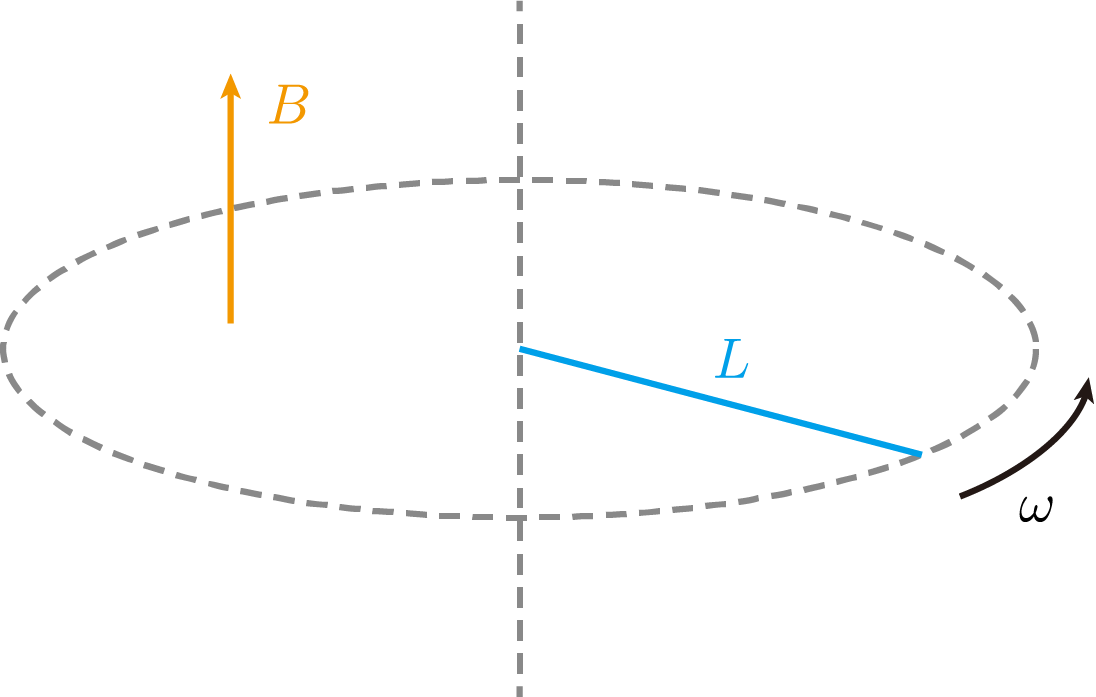
\includegraphics[width = 0.35\linewidth]{model_1}  & 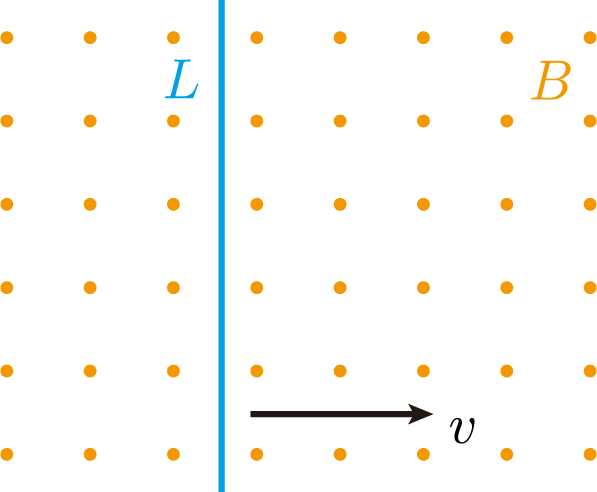
\includegraphics[width = 0.25\linewidth]{model_2} \\
     \mathscr E = \dfrac{1}{2} \omega B L^2  & \mathscr E = L v B 
\end{array}
\]


\section{电容器}

\renewcommand{\arraystretch}{2.5}
\begin{table}[H]
\centering
\makegapedcells
\begin{tabular}{c|c|c|c|c|c}
    \hline
    模型 & 平行板电容器 & 孤立导体球 & 球形$ ^{\text{1}} $ & 柱形$ ^{\text{1}} $ & 两根长直导线$ ^{\text{2}} $ \\
    
    \hline
    电容($ C $) & $ \dfrac{\varepsilon S}{d} $ & $ 4 \pi \varepsilon R $ & $ \dfrac{4 \pi \varepsilon R_1 R_2}{R_2 - R_1} $ & $ 2 \pi \varepsilon L \ln \dfrac{R_1}{R_2} $ & $ \pi \varepsilon \ln \dfrac{R}{d} $ \\

    \hline
\end{tabular}
\end{table}
注:
\begin{enumerate}
    \item $ R_1: $ 内径, $ R_2: $ 外径, $ R_2 > R_1 $
    \item $ R: $ 导线半径, $ d: $ 两导线距离
\end{enumerate}


\end{document}